\section{Hardware}
Der zweite wichtige Aspekt beim Aufbau eines unkonventionellen 
Supercomputers ist der physikalische Aufbau des Computers.
Hierbei muss man darauf achten ein Gleichgewicht zwischen den Faktoren: 
Energieverbrauch, Rechengeschwindigkeit und Kühlung zu finden.
Zusätzlich soll unabhängig von der Größe des Clusters eine
einfache Lösung für das Monitoring bereitgestellt werden.

\subsection{Hardwareauswahl und Motivation}
HIER NOCH INHALT EINFÜGEN! (wenn nicht redundant mit der Einleitung)


\subsection{Aufbau des Clusters}
Für ein Jetson-TK1-Cluster mit insulärer Stromversorgung
ist das Design des Racks der entschiedene Punkt um 
auch unter dauerhafter Höchstbelastung eine
stabile Funktion der Rechenknoten zu gewährleisten.
Durch die Verwendung eines Lithium-Ion-Akkus zur Energiespeicherung
und das Risiko eines Kurzschlusses durch Kondensionswasser muss
ein geschickt aufgebautes Rechencluster gewährleißten, dass die Temperatur
der gesamten Anlage in dem stark restringierten Bereich von 
$18^\circ\text{C}~\text{bis}~40^\circ \text{C}$ gehalten wird. 
%Besonders beim Aufbau eines insulären Jetson-TK1-Clusters ist die Kühlung ein
%heikles Thema, da sowohl die Temperatur des Rechenclusters als auch 
%die Temperatur des Energiespeichers in seinem stark restringierten Bereich liegen müssen.
\subsubsection{Anordnung der Rechenknoten}
Hinsichtlich der oben beschriebenen Problematik ist die Anordnung der Knoten 
das zentrale Instrument mit dem Man die Bildung potenzieller Wärmenester 
gegen den Platzverbrauch des Clusters abwägen kann.~\\
Wegen zu hoher Energiekosten muss auf den Einsatz einer
Wasserkühlung verzichtet werden um eine möglichst hohe Energieeffizienz 
er erreichen.
Die einfachsten Ansätze zum Aufbau des Supercomputers, 
welche sich mittels Luftkühlung umsetzen lassen, sind:
\begin{itemize}
\item[1)]Rechenknoten in horizontalen Schichten anzuordnen
\item[2)]Rechenknoten vertikal anzuordnen und nebeneinander aufstellen
\end{itemize} 
Je nach Aufbau ergeben sich dabei einige Vor- und Nachteile für den Großrechner, welche hier anhand der
Wärmebildern gezeigt werden.\\
~\\
\begin{minipage}{0.50\textwidth}
\centering
	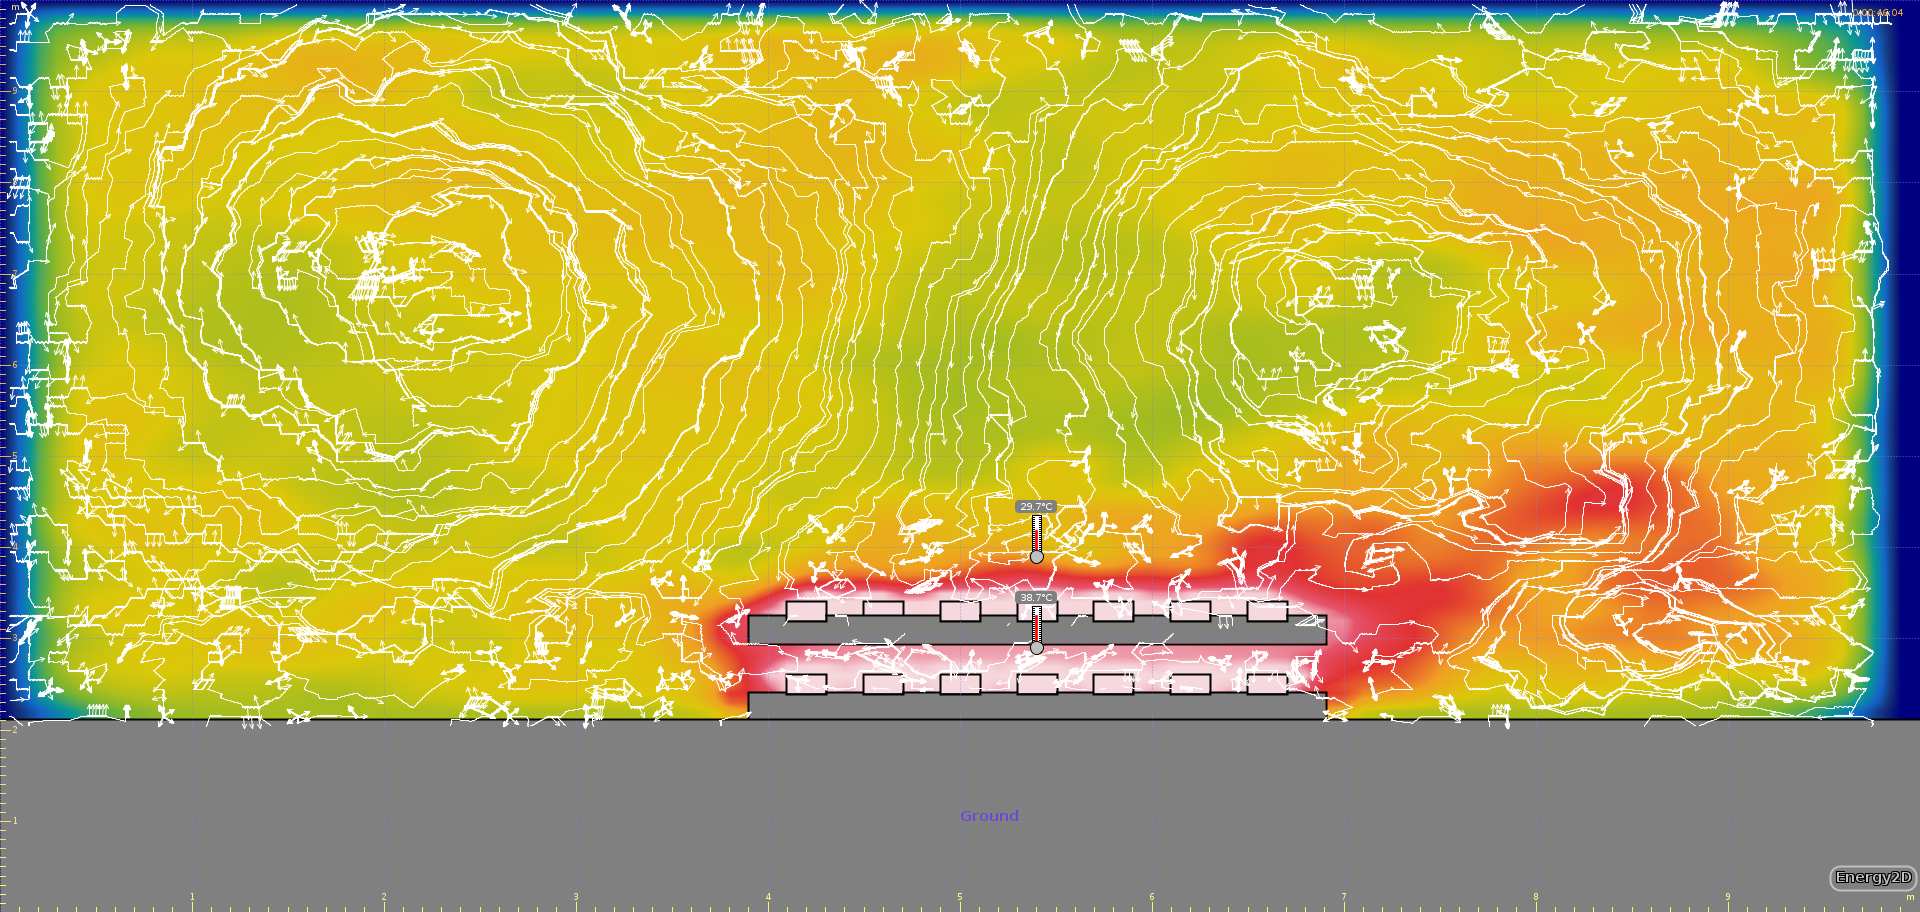
\includegraphics[width=0.99\textwidth]{./Bilder/Server-Aufbau/convective-horizontal-2.png}
	\captionof{figure}{Horizontaler Aufbau}
	\label{fig:sample_figure}
\end{minipage}
\hfill
\begin{minipage}{0.50\textwidth}
\centering
	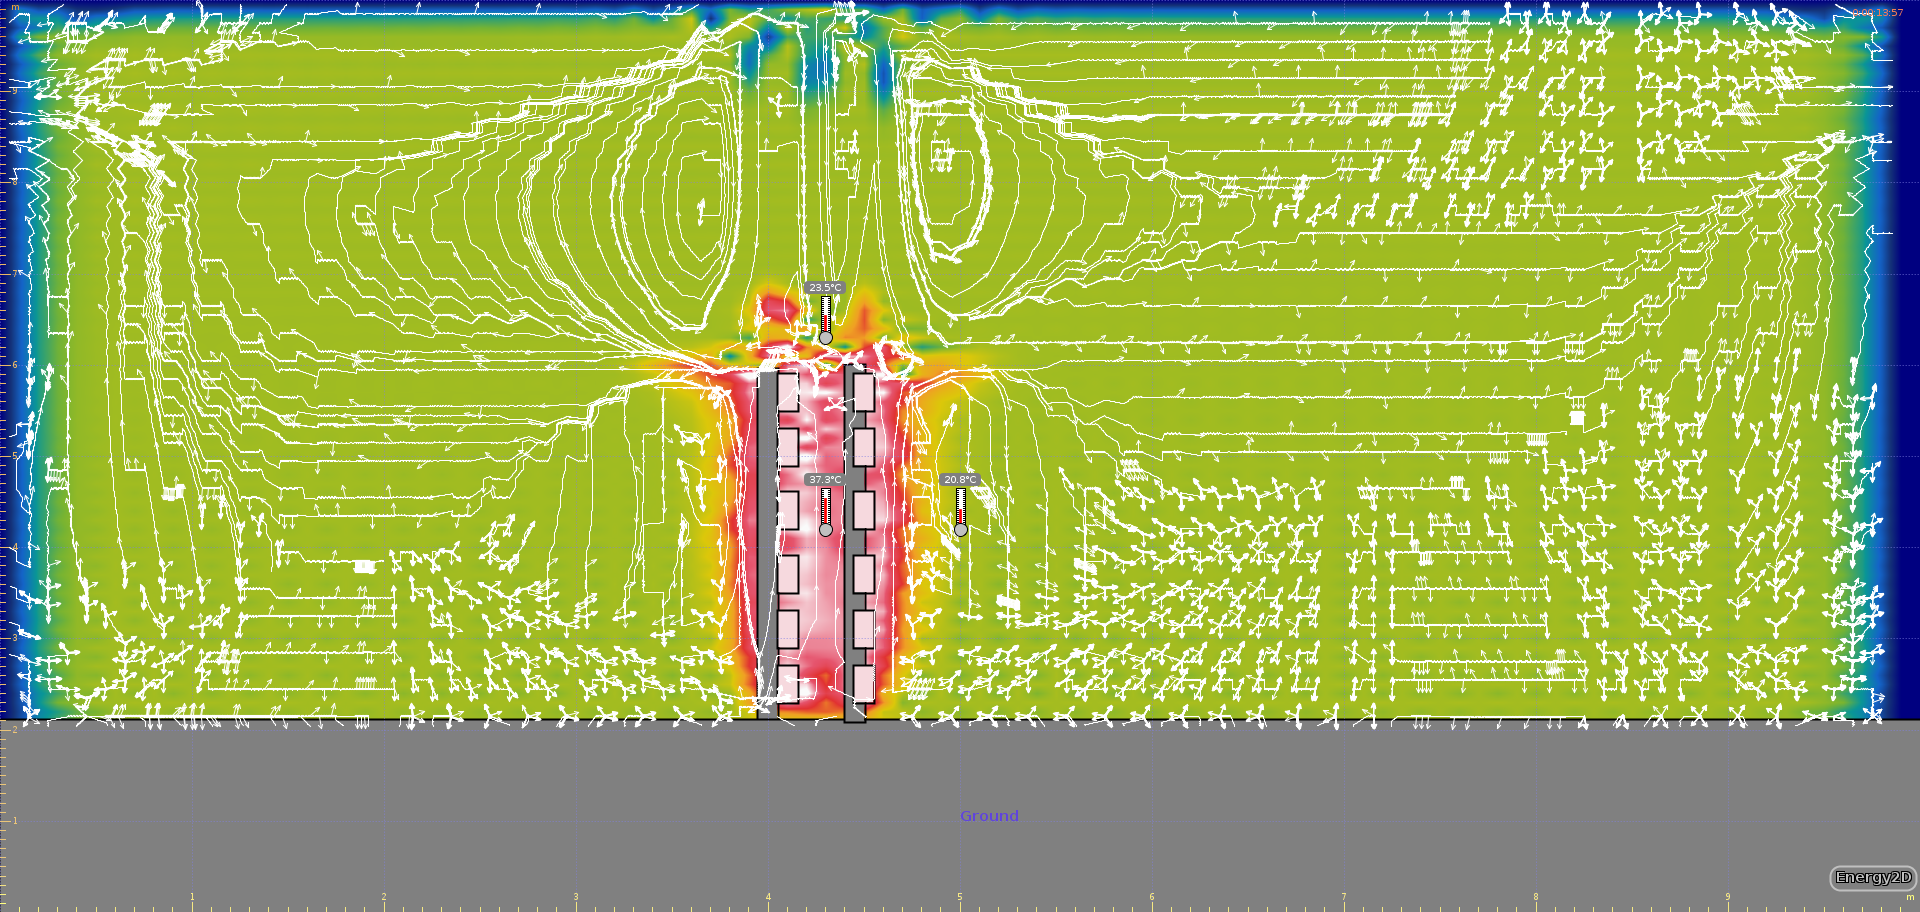
\includegraphics[width=0.99\textwidth]{./Bilder/Server-Aufbau/convective-vertical-2.png}
	\captionof{figure}{Vertikaler Aufbau}
	\label{fig:sample_figure}
\end{minipage}
~\\
Vergleicht man diese Beiden Ansätze, so sieht man, dass im horizontalen Szenario zwischen den 
Platten, auf denen die Rechenknoten angebracht sind, Wärme-Nester entstehen. Zudem liefert die
Analyse des Stromlinien Diagramms, dass besonders in der Mitte der Platten die Wärme nur schlecht  
abtransportiert werden kann.\\
Im Gegensatz dazu ist der Wärmeabtransport beim vertikalem Ansatz durch aufsteigende warme Luft
besser möglich. Hierbei sollte allerdings bemerkt werden, dass durch die schiefe Lage des Ventilators
die Gravitationskraft Unregelmäßigkeiten bei der Rotation verursachen könnte, was schlussendlich zu einer verkürzten Lebensdauer des Ventilators führen könnte.\\
Um die Vorteile der Beiden Ansätze zu kombinieren und gleichzeitig für Wartbarkeit des 
Rechenclusters zu erhöhen wählt man einen Ansatz, bei dem die Bords in einer Doppelhelix-Struktur 
angeordnet werden.\\
~\\
\begin{minipage}{0.50\textwidth}
\centering
	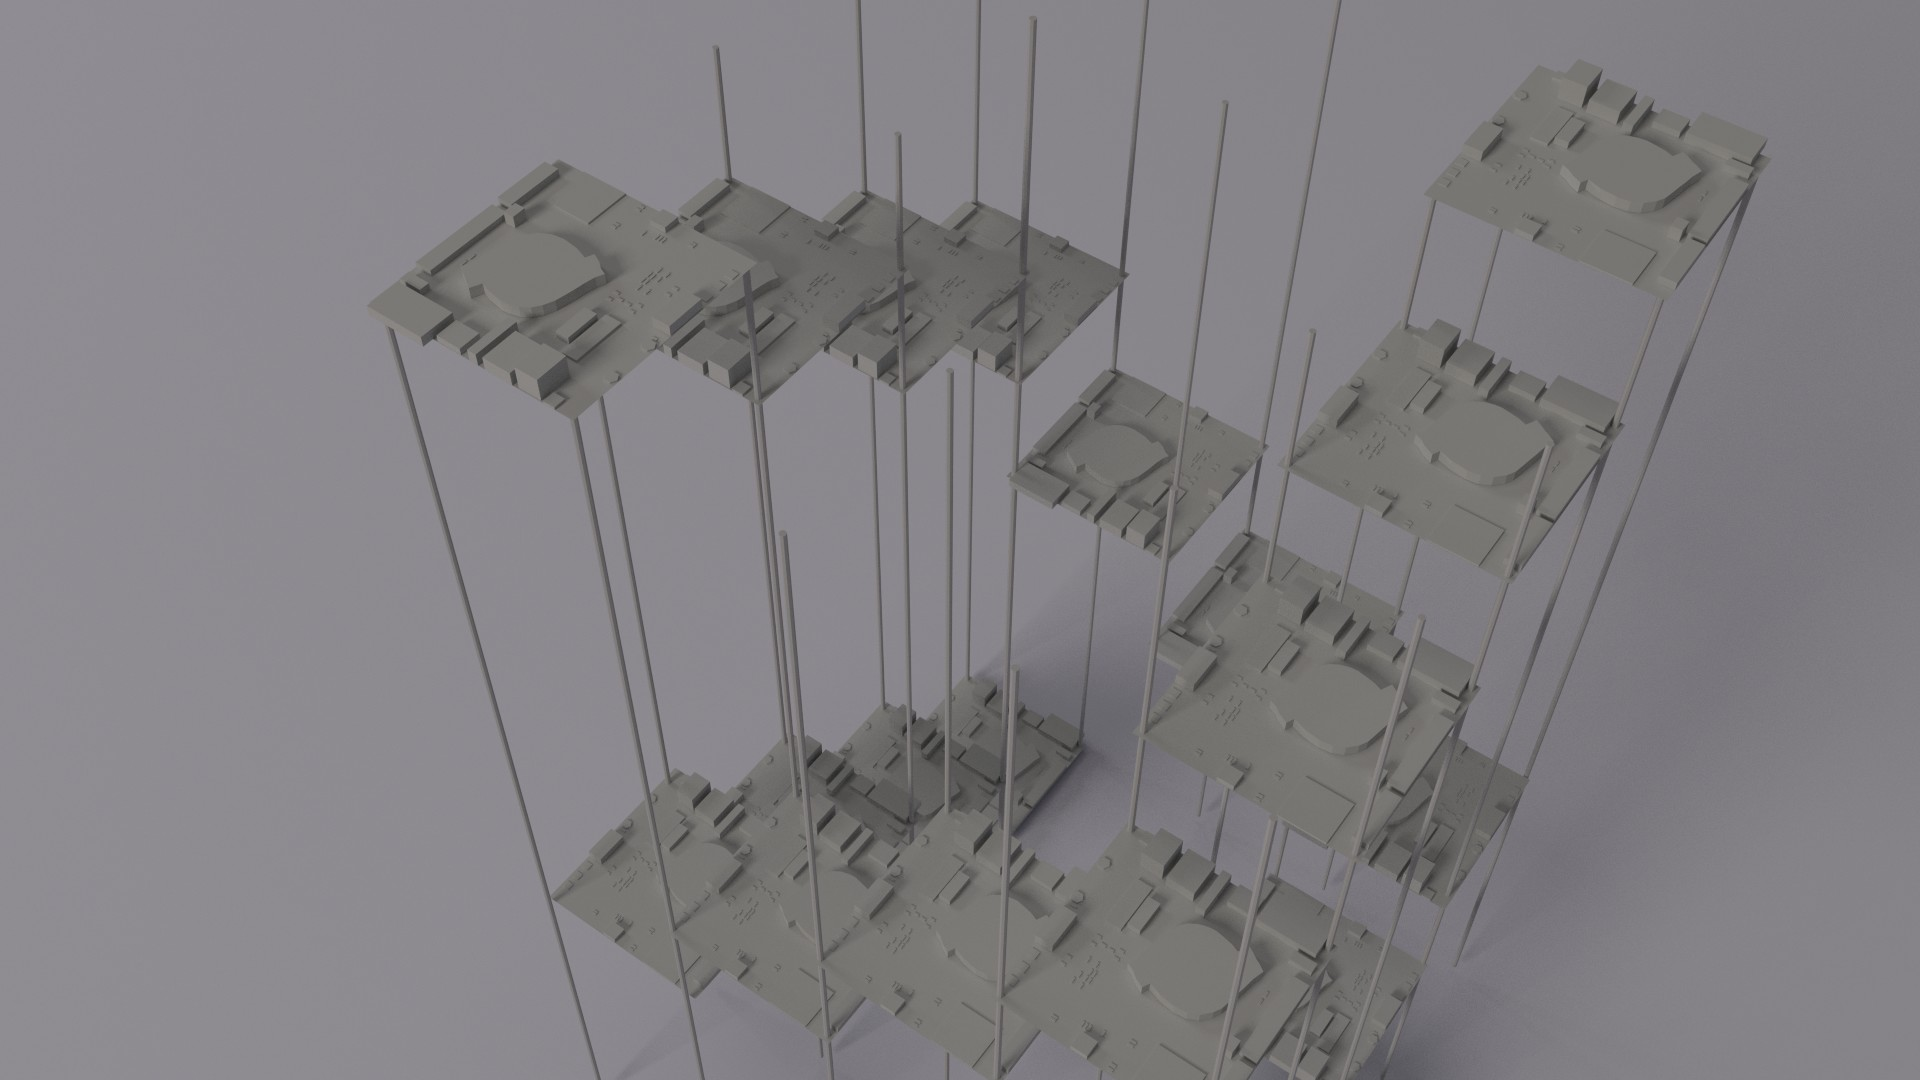
\includegraphics[width=0.99\textwidth]{./Bilder/Server-Aufbau/render3.jpg}
	\captionof{figure}{Render des Serveraufbaus}
	\label{fig:sample_figure}
\end{minipage}
\hfill
\begin{minipage}{0.50\textwidth}
\centering
	\includegraphics[width=0.99\textwidth]{./Bilder/Icarus/20160307_161232.jpg}
	\captionof{figure}{Serveraufbau (7. März 2016)}
	\label{fig:sample_figure}
\end{minipage}
~\\
Wie auf diesen Abbildungen zu erkennen ist wird durch die Verwendung der Doppelhelix-Struktur
ein größerer Abstand zwischen den Bords für eine verbesserte Kühlung, bei gleichzeitig geringem
Platzverbrauch ermöglicht.\\ 
\subsubsection{Strom und Netzwerkanbindung}
Über die Anordnung hinaus muss nun die Stromversorgung und die Netzwerkanbindung
der Bords geregelt werden. Eine besondere Herausforderung hierbei ist die 
Anordnung der Netzteile der einzelnen Rechenknoten. 
Um zu gewährleisten, dass sich durch das Aufheizen der Netzteile keine gefährlichen
Wärmenester bilden wird eine spezielle Halterung verwendet.
Unter nutzung moderner 3D-Druck Technologien, wie sind häufig in der 'Maker-Szene' eingesetzt werden,
wurde eine Halterung produziert, welche trotz geringem Materialaufwand eine sehr hohe stabiliät 
und eine gute Luftzufuhr ermöglicht.
\begin{minipage}{\textwidth}

\begin{center}
	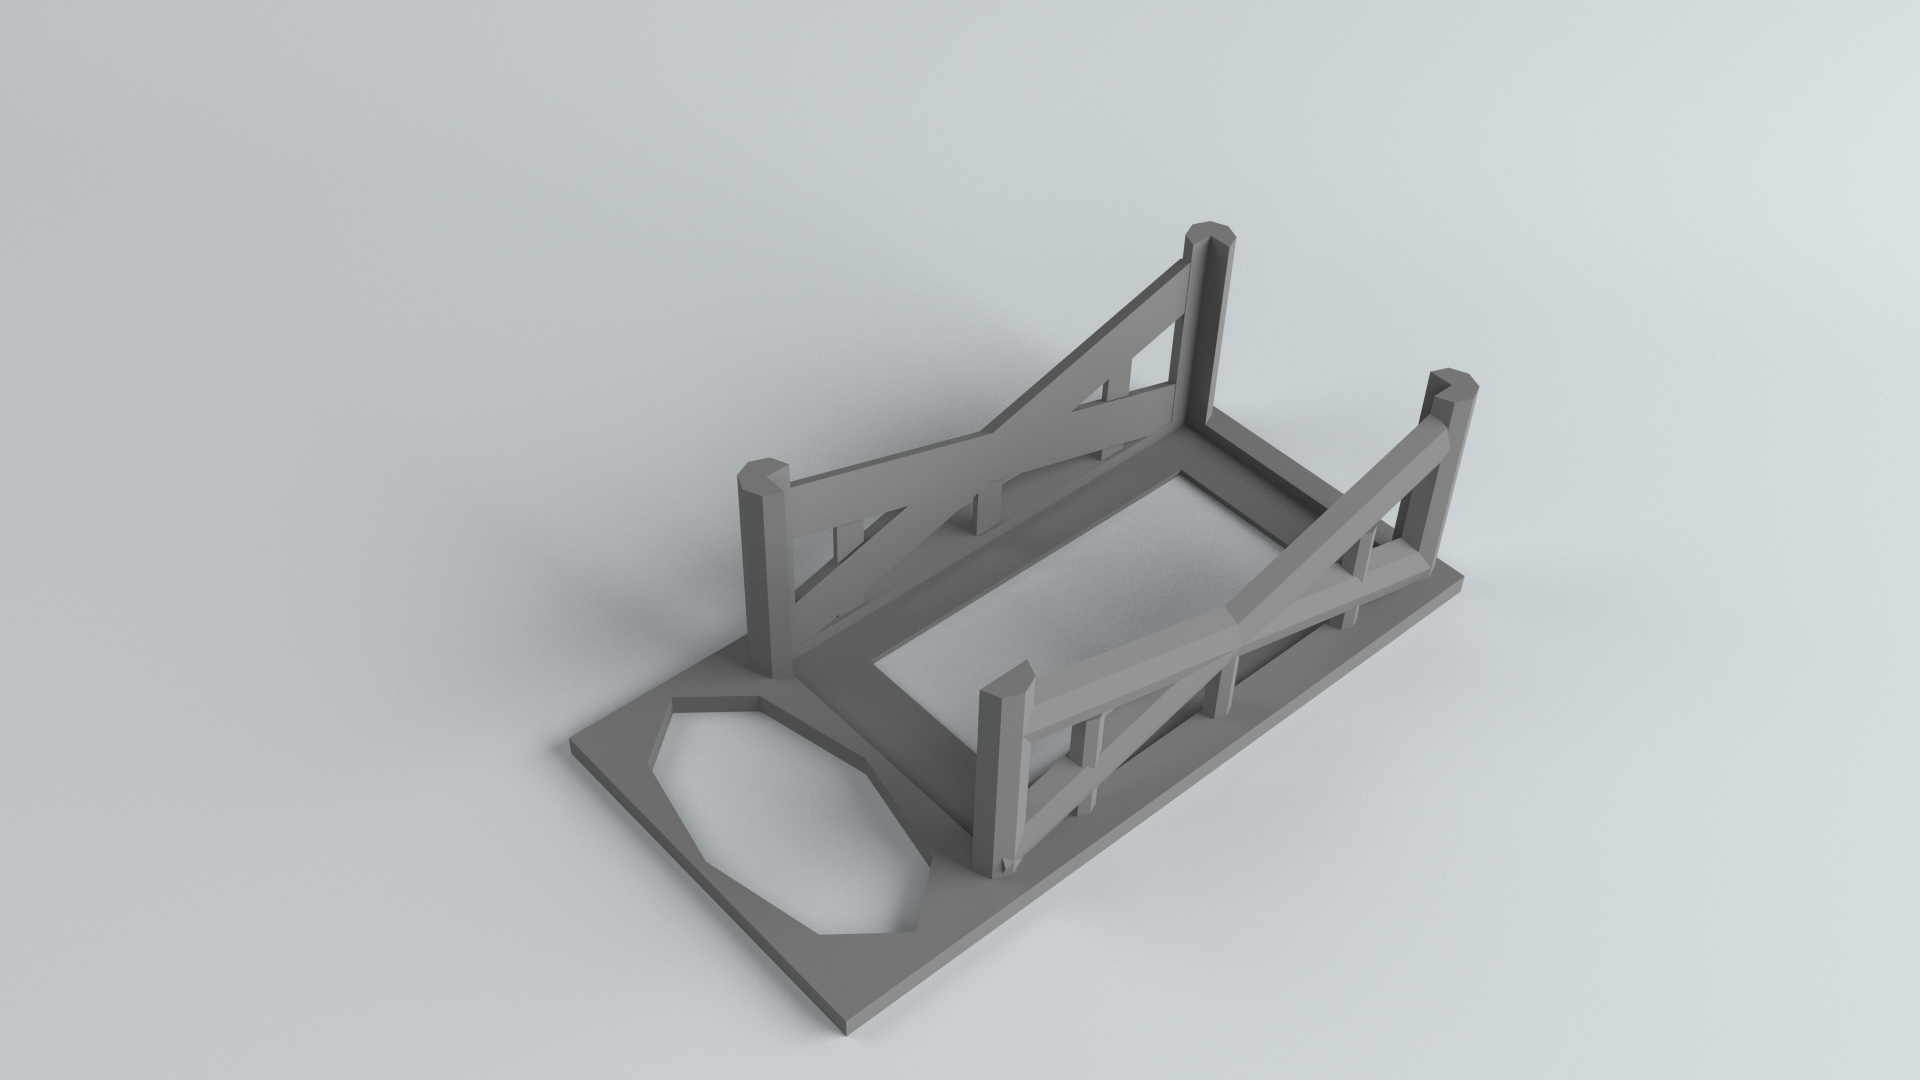
\includegraphics[width=0.7\textwidth]{./Bilder/Server-Aufbau/RenderPowerSupplyBox30.png}
		\captionof{figure}{Halterung für die Netzteile}
	\label{fig:sample_figure}

\end{center}	
\end{minipage}
~\\

Hinsichtlich des Aspektes 'Green-Computing' ist es wichtig ein Druck Filament zu verwenden, 
welche Bio-Kompatibel ist. Hierfür bietet sich der aus Mais-stärke gewonnene Biokunststoff PLA
(Polylactide) an. Polyacide hat einen Schmelzpunkt von $150^\circ\text{C}~\text{bis}~160^\circ \text{C}$
und ist daher ohne weiteres für die Halterung von Netzteilen verwendbar.


%\subsection{Wartung und Instandhaltung}
%\subsection{Dashboard} %(Ist gem dict.cc auch OK)
\subsection{Übersichtsseite}
Um das Monitoring und die Fernwartung des Clusters möglichst komfortabel zu bewerkstelligen wurde ein Dashboard eingerichtet. Hierfür ist ein RaspberryPi der ersten Generation ausreichend.
\subsubsection{Einrichtung Webserver}
Um die gemessenen Daten verwalten und darstellen zu können wird auf dem RaspberryPi ein LAMP-Server eingerichtet (Linux-Apache-MySQL-PHP). Die Daten werden folglich in der MySQL Datenbank abgespeichert und über PHP-Skripte ausgelesen und verarbeitet. Die Darstellung der Daten erfolgt mittel HTML, CSS und Javascript. Des Weiteren muss der RaspberryPi so konfiguriert werden, dass erstens das Webinterface von außen einsehbar ist , und vor allem, dass man von außen in die Datenbank schreiben kann.

\begin{minipage}{\textwidth}

\begin{center}
	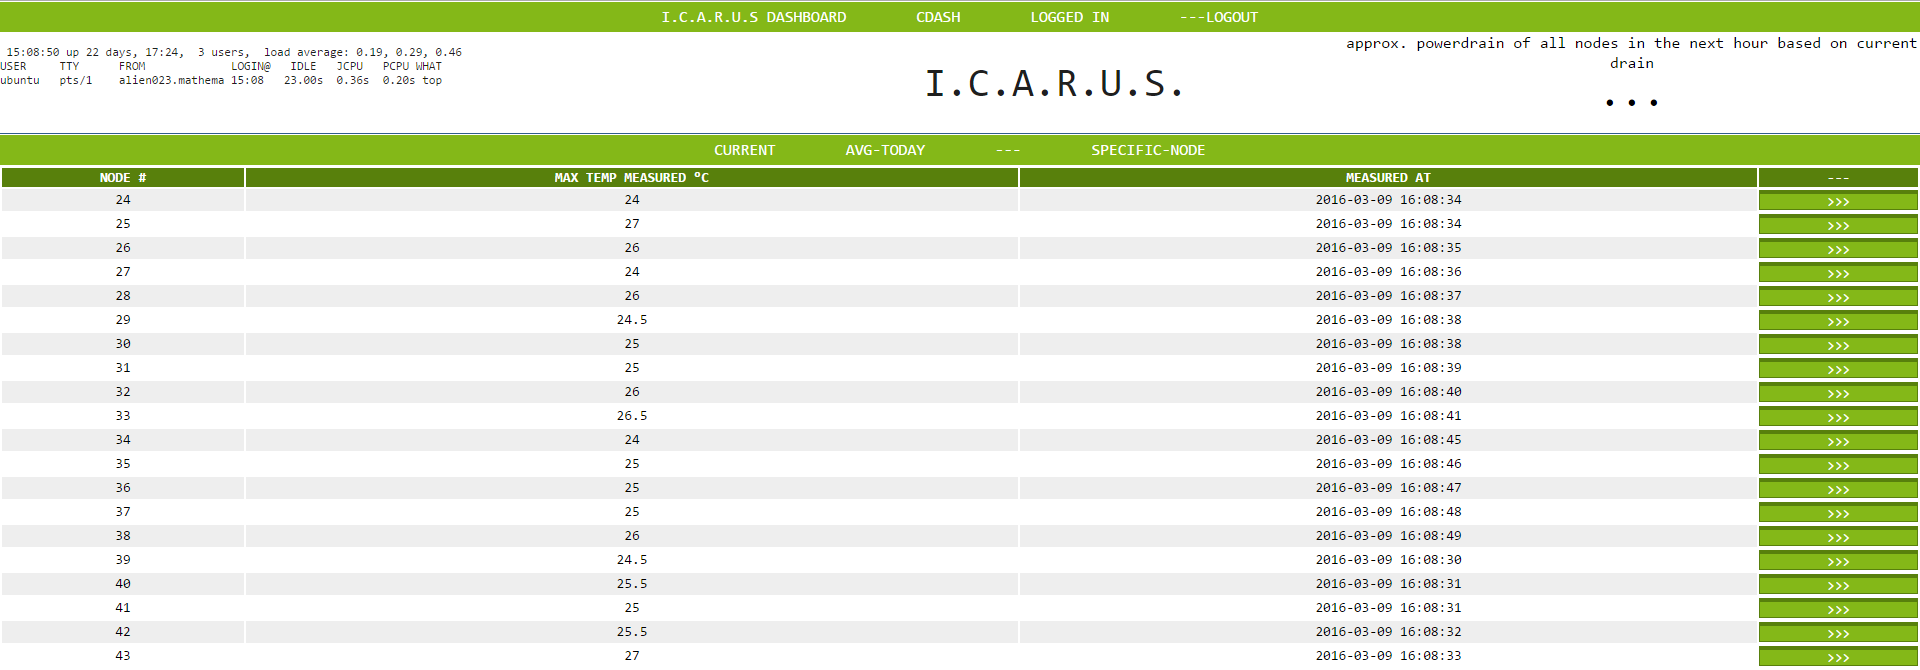
\includegraphics[width=0.7\textwidth]{./Bilder/Dashboard/Dashboard_frontend.png}
		\captionof{figure}{Dashboard Frontend}
	\label{fig:sample_figure}

\end{center}	
\end{minipage}

\subsubsection{Sammeln der Messdaten}
Die Temperaturen können lokal auf den einzelnen Boards ausgelesen werden. Dies wird verwendet um mittels C++ ein Programm laufen zu lassen, welches sich auf den einzelnen Rechenknoten nacheinander einloggt, die Temperatur Daten an verschiedenen Stellen des Jetson-Boards ausliest und anschließend eben jene in die MySQL-Datenbank auf dem Webserver einfügt.\\
Um die restringierte Hardware des Raspberry Pi's nicht zu überlasten wird das Programm auf dem Gateway-Knoten des Clusters ausgeführt, weshalb der oben Genannte Zugriff von außen des RaspberryPi's wichtig ist. \\
Um qualitative Aussagen über die Energieeffizienz machen zu können wurde eine PDU angeschafft, mit welcher man den Stromverbrauch der einzelnen Knoten messen können sollte. \\
--- HIER TEXT WARUM DAS MIT DER PDU NICHT GEHT ---\\
--- HIER TEXT BZGL NEUER MESSMETHODEN ---